\begin{task}[]{PCA}
 We use the data-set \text{iris.txt}. Each row in it has 4 Attributes and a label(classification).
 \begin{subtask}
 	We normalize the data, s.t. every Attribute has mean zero and variance 1. Therefore, for every column, we compute the sample mean and subtract it. Then, we devide by the standard deviation. Of course, this is only done for the columns containing attributes.
 	\begin{figure}[H]
 		\begin{lstlisting}[language=python]
	#3a
	n = len(iris)
	pre_iris = iris[:,0:4]
	pred = iris[:,4]
	mean = pre_iris.mean(0)
	step1 = pre_iris - mean
	standard_deviation=np.std(pre_iris, axis=0)
	normalized_data = np.multiply(step1, 1/standard_deviation).T   
 		\end{lstlisting}
 	\end{figure}
	\text{"normalized\_data"} does now contain one row per attribute, each row having mean zero and variance one.
\end{subtask}
\begin{subtask}
	We apply PCA on the normalized dataset. We plot a bar graph where the \text{i-th} bar shows how much of the original variance we already captured using the biggest \text{i} components.
\begin{lstlisting}[language=python]
def PCA(normalized_data):
	cov = np.cov(normalized_data)
	eigenvalues, eigenvectors = np.linalg.eig(cov)
	
	summe = np.sum(eigenvalues)
	eigenvalues_prop = eigenvalues/summe
	
	ind = [1,2,3,4]
	kum = np.zeros(4)
	kum[0] = eigenvalues_prop[0]
	for i in range(1,4):
		kum[i]=kum[i-1] + eigenvalues_prop[i]  
	kum=kum*100
	plt.bar(ind, kum)
	rounded=np.round(kum,2)
	for idx,y in enumerate(rounded):
	plt.text(ind[idx]-0.2,y+1,str(y)+"%")
	plt.show()    
	return eigenvalues, eigenvectors
\end{lstlisting}
Calling the function produces the following plot:
\begin{figure}[H]
	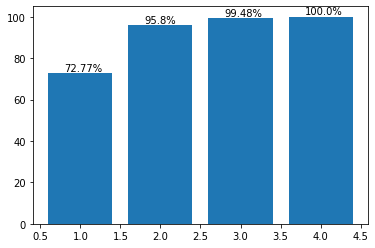
\includegraphics[]{bar}
\end{figure}
We see that for two components we explained already more than 95\% of the variance.
\end{subtask}
\begin{subtask}
	We do the PCA for the two biggest components. We wrote the following function:
\begin{lstlisting}[language=python]
	def threec(eigenvalues, eigenvectors, normalized_data, pred):
		B = eigenvectors[:,0:2]
		normalized_data_p = np.matmul(B.T, normalized_data)
		normalized_data_p = np.vstack((normalized_data_p, pred))
		colors = ['red','green','blue']
		plt.scatter(normalized_data_p[0], normalized_data_p[1], 
			c=normalized_data_p[2], cmap=matplotlib.colors.ListedColormap(colors))
		return
\end{lstlisting}
The first input arguments are clear, in the last argument we give the real data values from iris.txt just without the classification column. We then used the first two eigenvalues for projection on the $R^2$. Calling it, we get
\begin{figure}[H]
		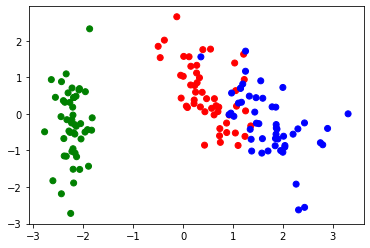
\includegraphics[]{2dprojectionPCA}
\end{figure}
where we used different colors for different classes(red=Setosa,green=Versicolour,blue=Virginica). We observe, that the green dots are well separated from the rest. Therefore we can argue, that Versicolour is pretty unique compared to the other two. For the red and blue dots it can be harsh to find a good decision boundary around x=1 we got both blue and red samples. The Setosa and the Virginica data seem to have more in common. Though, if we go away from the boundary, we could use the points to get - at least on the given training data - a very clear classification.
\end{subtask}
\begin{subtask}
We perform the PCA for n=1,2,3,4 components. Then we take the computed points from $R^{n}$ and embed them in $R^4$ to calculate an error distance. Doing this, we need to consider the normalization we have on our \text{normalized\_data}, which was, for real dataset X with mean $\bar{x}$ and variance $\text{std}^2$ 
\begin{align*}
normalized\_data=\frac{X-\bar{x}}{std}\\
\end{align*}
Following the idea of slide 27 in lecture 10, we get
\begin{align*}
a^n&=B^T\cdot\left( X-\bar{x}\right) \\&= B^T\cdot\left( normalized\_data \cdot std\right) \\
\\
\tilde{x}^n&=\bar{x}+B\cdot a^n
\end{align*}
where B is the matrix of the first n eigenvalues. We implemented this backtransformation in the comp\_set function.
\begin{lstlisting}[language=python]
def comp_set(n, eigenvectors, normalized_data, mean, var):
	B = eigenvectors[:,0:n+1]
	normalized_data_p = np.matmul(B.T, normalized_data) 
	reconstruction = np.matmul(B, normalized_data_p)
	rec=np.multiply(reconstruction.T,var)
	rec=rec+mean
	return rec
\end{lstlisting}
Now, we can compare the backtransformed data to the original uncompressed data via normalized mean squared error.
\begin{lstlisting}[language=python]
def rmse(x):
	return np.sqrt(np.mean(x**2))

def threed(eigenvalues, eigenvectors, normalized_data, pre_iris, mean, var):
	lsg=np.zeros([4,4])
	for comp in range(4):
		re = comp_set(comp, eigenvectors, normalized_data, mean, var)
		diff = re - pre_iris
	for feature in range(4):
		lsg[comp,feature]=rmse(diff[:,feature])/
			(np.sum(pre_iris[:,feature]/len(pre_iris)))
	print("lsg:", lsg)
	return 
\end{lstlisting}
Calling the threed function gives us the following solution:
\begin{table}[H]
	\begin{tabular}{lllll}
		& x\_1    & x\_2     & x\_3    & x\_4     \\
		n=1 & 6.406\% & 12.641\% & 6.021\% & 16.642\% \\
		n=2 & 3.945\% & 1.339\%  & 5.946\% & 16.158\% \\
		n=3 & 0.531\% & 0.252\%  & 5.381\% & 4.769\%  \\
		n=4 & 0       & 0        & 0       & 0       
	\end{tabular}
\end{table}
\end{subtask}
\begin{subtask}
	\begin{enumerate}
		\item
	Whitening is a technique to remove redundancies in our data. This is done by analyzing correlations between features and their variances. The covariance matrix $\Sigma$ is very important in doing so, because if $\Sigma$ is an identity matrix, we have no correlation between the features at all and every feature has normed variance of 1 which is the desired case for running stable algorithms on the data. In this case we call the dataset $\tilde{x}$ whitened. Because the resulting data is not unique, we can think of a somewhat 'best' transformation that still fits the requirements. The practical difference between PCA and ZCA lies in the interpretation of 'best' in the last sentence. Both are interested in normalizing the covariance as described, the PCA does this while also compressing the data. On the other hand, the ZCA is the better approach if we want to keep the new data pretty close to the original. We get it pretty easy from the PCA by multiplying an orthogonal matrix R from the left. The result still has the identity as covariance matrix. Choosing R as the matrix of eigenvectors from $\Sigma$ will turn out to be optimal. We then call the matrix product $R\cdot\tilde{x}$ ZCA-whitened. Literature isn't clear about normalizing w.r.t. the means though. In 2. we give the idea of computation after normalization w.r.t. the mean, but e.g. brunner ( see \text{"https://cbrnr.github.io/2018/12/17/whitening-pca-zca/"}) does not normalize the means, but still gets effective results.
	\item
	First of all we need to normalize every attribute of x, s.t. it has mean 0. We therefore estimate the mean by the sample mean $\hat{x}$:
	\begin{align*}
	x^* = x - \hat{x}=x-\frac{1}{n}\sum_{i=1}^n x_i
	\end{align*}
	We compute the covariance matrix via
	\begin{align*}
	\Sigma=\frac{1}{n}\sum_{i=1}^{n} (x-\hat{x})^T (x-\hat{x})=\frac{1}{n}\sum_{i=1}{n} x^{*T} x^{*}
	\end{align*}
	and calculate an singular value decomposition $\Sigma=USV$, because we need the eigenvalues(now stored in S) and the eigenvectors (now stored in the columns of U). With this all done, we can compute the PCA whitened data:
	\begin{align*}
	x^{\text{PCAw}}=diag((diag(S)+\epsilon)^{-0.5})\cdot U^T\cdot x*
	\end{align*}
	where $diag$ extracts the diagonal of a matrix, or constructs a diagonal matrix given a vector.
	Finally, we can derive the ZCA via:
	\begin{align}\label{zca}
	x^{\text{ZCAw}}=U\cdot x^{\text{PCAw}}
	\end{align}
	\item
	If we are given a new data example x, it will change the mean and therefore all parameters. In case we got big data we can assume that the single data point x has low impact on the mean and the computed covariance matrix. Then it is sufficient to use \ref{zca} for the single observation vector x and append the resulting column to $x^{\text{ZCAw}}$. \\
	\item The following pyhton implementation follows the approach without normalization like presented in the webpage from brunner:
	\begin{lstlisting}[language=python]
def zca_brunner(x,epsilon):
	if x.shape[0]>x.shape[1]:
		raise
	evals,evecs=np.linalg.eigh(np.cov(x))
	evals=evals+epsilon
	z = evecs @ np.diag(evals**(-1/2)) @ evecs.T @ x
	return z
	\end{lstlisting}
	Alternatively, we could normalize with the mean and get
	\begin{lstlisting}[language=python]
def zca_whitening(epsilon):
	pre_iris = iris[:,0:4]
	mean = pre_iris.mean(0)
	xstern = (pre_iris - mean).T
	cov = np.cov(xstern)
	eigenvalues, eigenvectors = np.linalg.eigh(cov)
	xPCAwhite=np.diag(1./np.sqrt(eigenvalues+epsilon))@eigenvectors.T@xstern
	xZCAwhite=eigenvectors@xPCAwhite
	return xZCAwhite
	\end{lstlisting}
	\end{enumerate}
\end{subtask}
\end{task}


